\documentclass[../psets.tex]{subfiles}

\pagestyle{main}
\renewcommand{\leftmark}{Problem Set \thesection}
\setcounter{section}{3}

\begin{document}




\section{Applications of Fraction Rings}
Throughout this assignment, $R$ will denote a \emph{commutative} ring.
\begin{enumerate}
    \item \marginnote{2/1:}Let $R$ be a ring, and let $f\in R$ be an element which is not a zero divisor. Recall that we defined $R_f=D^{-1}R$ for $D=\{1,f,f^2,\dots\}$. Prove that
    \begin{equation*}
        R_f \cong R[X]/(fX-1)
    \end{equation*}
    using the universal property of the ring of fractions.
    \item Let $\Z[i]=\Z[X]/(X^2+1)$ denote the ring of \textbf{Gaussian integers}. Recall from class that $\Z[i]$ is a Euclidean domain with norm $N:\Z[i]\to\Zg$ defined by $N(a+bi)=a^2+b^2$.
    \begin{enumerate}[label={(\alph*)}]
        \item Let $R$ be a Euclidean domain with norm $N$ which satisfies $N(xy)=N(x)N(y)$ for all $x,y\in R$. Prove that $a\in R$ is a unit iff $N(a)=1$. (Hint: Start by computing $N(1)$.)
        \item Using part (a), find the units in $\Z[i]$.
        \item Prove that $\Frac(\Z[i])=\Q[i]$.
    \end{enumerate}
    \item 
    \begin{enumerate}[label={(\alph*)}]
        \item For $a,b\in\Z$, prove that $a^2-2b^2=0$ iff $a=b=0$.
        \item Prove that $\Q[\sqrt{2}]=\Q[X]/(X^2-2)$ is a field.
    \end{enumerate}
    \item Let $D$ be a multiplicative subset of an integral domain $R$. Now $R$ is a subring of $D^{-1}R$. Let $J$ be an ideal of $D^{-1}R$. Put $I=R\cap J$.
    \begin{enumerate}[label={(\alph*)}]
        \item Is $I$ an ideal of $R$?
        \item Prove that if $I\neq R$, then $I\cap D=\emptyset$.
        \item Let $b\in J$. Is it true that $b=d^{-1}a$ for some $d\in D$ and $a\in I$?
        \item Prove that if $I$ is an ideal in $R$, then $I^e=\{s^{-1}x\in D^{-1}R\mid s\in D,\ x\in I\}$ is an ideal in $D^{-1}R$.
        \item Using part (c), prove that if $J$ is an ideal of $D^{-1}R$, then $J=(R\cap J)^e$. Therefore, we have a surjective map of sets
        \begin{equation*}
            \{\text{Ideals in }R\} \to \{\text{Ideals in }D^{-1}R\}
        \end{equation*}
        given by $I\mapsto I^e$. Note that the right inverse is given by $J\mapsto R\cap J$. Is this map a bijection?
        \item If $R$ is a PID, is $D^{-1}R$ a PID?
    \end{enumerate}
    \item 
    \begin{enumerate}[label={(\alph*)}]
        \item Let $D=\{n\in\Z:2\nmid n\}$. Recall that we defined
        \begin{equation*}
            \Z_{(2)} = D^{-1}R
            = \{a/b\in\Q:2\nmid b\}
        \end{equation*}
        Write down all of the ideals in $\Z_{(2)}$. You can use the fact that the ideals in $\Z$ are $(n)=n\Z$ for $n\in\Z$, and the previous question. Which of these ideals are maximal? For each maximal ideal $M\in\Z_{(2)}$, what is the field $\Z_{(2)}/M$?
        \item Let $D=\{2^n\mid n\in\Zg\}$ and let $R=D^{-1}\Z$. Write down the ideals in $R$. Which of these ideals are maximal?
    \end{enumerate}
    \item 
    \begin{enumerate}[label={(\alph*)}]
        \item Define $M_2:\{\text{commutative rings}\}\to\{\text{sets}\}$ by
        \begin{equation*}
            M_2(R) = \left\{
                \begin{pmatrix}
                    a & b\\
                    c & d\\
                \end{pmatrix}
                \mid a,b,c,d\in R
            \right\}
        \end{equation*}
        Show that for any $R$, there is a natural bijection between the set $M_2(R)$ and the set $S_1$ of ring homomorphisms between $\Z[X,Y,Z,W]$ and $R$. Note that notationally,
        \begin{equation*}
            S_1 = \text{Hom}_\text{ring}(\Z[X,Y,Z,W],R)
        \end{equation*}
        One sometimes says that $\Z[X,Y,Z,W]$ represents the function $M_2$.
        \item (\textbf{You do not need to turn in part (b)}, but you are encouraged to think about it.)\par
        Actually, $M_2(R)$ can be naturally given a ring structure: Addition and multiplication are defined using the same procedure as $M_2(\R)$ (or with any other field you may have seen). Hence, it makes sense to talk about the units of $M_2(R)$.\par
        Define the set $GL_2(R)$ to be the units of $M_2(R)$, i.e.,
        \begin{equation*}
            GL_2(R) = M_2(R)^\times
        \end{equation*}
        Show that for any $R$, there is a natural bijection between $GL_2(R)$ and the set $S_2$ defined by
        \begin{equation*}
            S_2 = \text{Hom}_\text{ring}(\Z[X,Y,Z,W]_{XW-YZ},R)
        \end{equation*}
        Note that $\Z[X,Y,Z,W]_{XW-YZ}$ denotes the \textbf{localization} of $\Z[X,Y,Z,W]$ by the multiplicative set generated by $XW-YZ$ (that is, the multiplicative set $(1,XW-YZ,(XW-YZ)^2,\dots)$). (Hint: Use the universal property.)\par
        One sometimes says $\Z[X,Y,Z,W]_{XW-YZ}$ represents the function $GL_2$.
        % \begin{proof}
        %     XW-YZ is like the determinant.
        % \end{proof}
    \end{enumerate}
    \item Let $\Q(X)$ denote the field of fractions of $\Q[X]$. By the universal property of a polynomial ring, we know that giving a ring homomorphism $\varphi:\Q[X]\to\R$ is equivalent to choosing an element $r\in\R$ and setting $\varphi(X)=r$. Which ring homomorphisms $\varphi:\Q[X]\to\R$ extend to ring homomorphisms $\tilde{\varphi}:\Q(X)\to\R$? These ring homomorphisms should satisfy the following commutative diagram.
    \begin{center}
        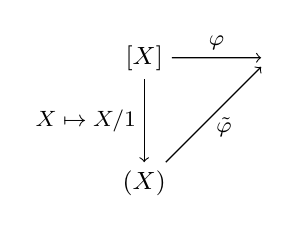
\begin{tikzpicture}[scale=1.6]
            \small
            \node (pols) at (0,1) {$\Q[X]$};
            \node (frcs) at (0,0) {$\Q(X)$};
            \node (R)    at (1,1) {$\R$};
    
            \footnotesize
            \draw [->] (pols) -- node[left]            {$X\mapsto X/1$}    (frcs);
            \draw [->] (frcs) -- node[below right=-2pt]{$\tilde{\varphi}$} (R);
            \draw [->] (pols) -- node[above]           {$\varphi$}         (R);
        \end{tikzpicture}
    \end{center}
    \item $F$ is a field. Let $R$ be the smallest subring of $F[X]$ such that (a) $F\subset R$ and (b) both $X^2$ and $X^3$ belong to $R$.
    \begin{enumerate}[label={(\alph*)}]
        \item Use the identity $(X^2)^3=(X^3)^2$ to deduce that $R$ is \emph{not} a UFD.
        \item Exhibit an ideal $I$ of $R$ that is not a principal ideal.
    \end{enumerate}
    \item Mimic Euclid's proof of the infinitude of primes in $\Z$ to show that $F[X]$ has infinitely many primes for every field $F$.
    \item Let $R$ be an integral domain and let $d$ be the degree of a nonzero $f\in R[X]$. Prove that $\{a\in R\mid f(a)=0\}$ is finite. \emph{Hint}: Case 1 --- first prove this when $R$ is a field. Case 2 --- reduce to case 1 by looking at the fraction field of $R$.
\end{enumerate}




\end{document}